% The 5 x 5 optimum: (a) the grid, (b) its row-column incidence graph,
% (c) the 8 optima, one orbit of the dihedral group.
\begin{figure}[t]
\centering
\begin{tikzpicture}[scale=0.82,
  blk/.style={circle,fill=black,inner sep=0pt,minimum size=7pt},
  kpt/.style={circle,draw=black!70,fill=white,inner sep=0pt,minimum size=7pt},
  cyc/.style={line width=2.2pt,draw=cyccol,line join=round},
  pen/.style={line width=1.4pt,draw=pencol,dash pattern=on 3pt off 2pt}]
  % ---------- (a) the grid ----------
  \begin{scope}
    % kept blocks
    \fill[keptcol,rounded corners=6pt] (0.55,-0.55) -- (2.45,-0.55) -- (2.45,-2.45)
      -- (1.45,-2.45) -- (1.45,-3.45) -- (0.55,-3.45) -- cycle;
    \fill[keptcol,rounded corners=6pt] (3.55,-1.55) -- (5.45,-1.55) -- (5.45,-4.45)
      -- (4.45,-4.45) -- (4.45,-5.45) -- (1.55,-5.45) -- (1.55,-4.55) -- (2.55,-4.55)
      -- (2.55,-3.55) -- (3.55,-3.55) -- cycle;
    \draw[black!15] (1,-1) grid (5,-5);
    % the 8-cycle as a closed rook tour through black points
    \draw[cyc] (3,-1) -- (5,-1) -- (5,-5) -- (1,-5) -- (1,-4) -- (2,-4) -- (2,-3)
      -- (3,-3) -- cycle;
    \foreach \x/\y in {1/1,2/1,1/2,2/2,4/2,5/2,1/3,4/3,5/3,3/4,4/4,5/4,2/5,3/5,4/5}
      \node[kpt] at (\x,-\y) {};
    \foreach \x/\y in {3/1,5/1,2/3,3/3,1/4,2/4,1/5,5/5}
      \node[blk] at (\x,-\y) {};
    \foreach \x/\y in {4/1,3/2}
      \node[blk,fill=pencol] at (\x,-\y) {};
    \foreach \i in {1,...,5} {
      \node[font=\scriptsize,black!70] at (\i,-0.35) {$c_{\i}$};
      \node[font=\scriptsize,black!70] at (0.3,-\i) {$r_{\i}$};
    }
    \node[font=\small] at (3,-6.1) {(a) the blackout};
  \end{scope}
  % ---------- (b) the incidence graph ----------
  \begin{scope}[xshift=9.6cm,yshift=-3cm]
    \def\R{1.75}
    \foreach \lab/\ang in {r_1/112.5,c_5/67.5,r_5/22.5,c_1/-22.5,r_4/-67.5,
                           c_2/-112.5,r_3/-157.5,c_3/157.5}
      \coordinate (\lab) at (\ang:\R);
    \coordinate (c_4) at ($(r_1)+(100:1.15)$);
    \coordinate (r_2) at ($(c_3)+(205:1.1)$);
    \draw[cyc] (r_1)--(c_5)--(r_5)--(c_1)--(r_4)--(c_2)--(r_3)--(c_3)--cycle;
    \draw[pen] (r_1)--(c_4);
    \draw[pen] (c_3)--(r_2);
    \foreach \lab in {r_1,r_2,r_3,r_4,r_5}
      \node[draw,fill=white,rectangle,inner sep=1.5pt,minimum size=13pt,font=\scriptsize]
        at (\lab) {$\lab$};
    \foreach \lab in {c_1,c_2,c_3,c_4,c_5}
      \node[draw,fill=white,circle,inner sep=0.5pt,minimum size=14pt,font=\scriptsize]
        at (\lab) {$\lab$};
    \node[font=\small] at (0,-3.1) {(b) the graph $G_S$};
  \end{scope}
\end{tikzpicture}

\medskip
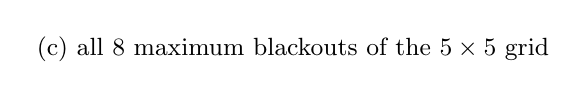
\begin{tikzpicture}[scale=0.23]
  % (c) the orbit; each pattern lists the rows top to bottom, 1 = blacked out
  \minigrid{0}{{0,0,1,1,1},{0,0,1,0,0},{0,1,1,0,0},{1,1,0,0,0},{1,0,0,0,1}}
  \minigrid{7.5}{{0,0,0,1,1},{0,0,1,1,0},{1,1,1,0,0},{1,0,0,0,0},{1,0,0,0,1}}
  \minigrid{15}{{1,0,0,0,1},{0,0,0,0,1},{0,0,1,1,1},{0,1,1,0,0},{1,1,0,0,0}}
  \minigrid{22.5}{{1,0,0,0,1},{0,0,0,1,1},{0,0,1,1,0},{0,0,1,0,0},{1,1,1,0,0}}
  \minigrid{30}{{1,0,0,0,1},{1,0,0,0,0},{1,1,1,0,0},{0,0,1,1,0},{0,0,0,1,1}}
  \minigrid{37.5}{{1,0,0,0,1},{1,1,0,0,0},{0,1,1,0,0},{0,0,1,0,0},{0,0,1,1,1}}
  \minigrid{45}{{1,1,0,0,0},{0,1,1,0,0},{0,0,1,1,1},{0,0,0,0,1},{1,0,0,0,1}}
  \minigrid{52.5}{{1,1,1,0,0},{0,0,1,0,0},{0,0,1,1,0},{0,0,0,1,1},{1,0,0,0,1}}
  \node[font=\small] at (30,-7.4) {(c) all 8 maximum blackouts of the $5\times5$ grid};
\end{tikzpicture}
\caption{The $5\times5$ optimum. (a) The 10 blacked-out points (filled) and the 15 kept points
(open), which form the 2 shaded blocks of 5 and 10. The bold closed path turns only at black
points and runs alternately along rows and columns; its 8 corners are the 8-cycle of (b). The 2
grey black points are the 2 pendant edges of (b).
(b) The same blackout as a graph: one vertex for each row and each column, and an edge
$r_jc_i$ for each black point $(i,j)$. It is an 8-cycle with 2 pendant edges. A valid blackout can
have no 4-cycle and no 6-cycle (Lemma~\ref{lem:girth}), so 8 is the shortest cycle allowed.
(c) The 8 maximum blackouts. They are the images of (a) under the 8 symmetries of the square, and
no 2 of them coincide.}
\label{fig:fivefive}
\end{figure}
